
 \cajita{%
Población con gastos inferiores a la línea de pobreza extrema}%
{%
 Este indicador muestra el porcentaje de población cuyo consumo es inferior a la línea de pobreza extrema\footnote{Para 2014, este valor era de Q 5,750 por persona al año.}, es decir, corresponde al grupo de población que no logra cubrir el costo del consumo mínimo de alimentos. 
 
En la gráfica se advierte que entre 2000 y 2006,  la pobreza extrema se mantuvo casi  al mismo nivel; no obstante en  2014 se observó un aumento de 8.2 puntos porcentuales.}%
{%
 Proporción de partos con asistencia de médico o ginecólogo} %
{%
 Républica de Guatemala, Encovi 2000, 2006 y 2014, en quetzales de cada año} %
{%
 \begin{tikzpicture}[x=1pt,y=1pt]  % Created by tikzDevice version 0.7.0 on 2015-11-27 14:11:58
% !TEX encoding = UTF-8 Unicode
\definecolor[named]{fillColor}{rgb}{1.00,1.00,1.00}
\path[use as bounding box,fill=fillColor,fill opacity=0.00] (0,0) rectangle (289.08,198.74);
\begin{scope}
\path[clip] (  0.00,  0.00) rectangle (289.08,198.74);

\path[] (  0.00,  0.00) rectangle (289.08,198.74);
\end{scope}
\begin{scope}
\path[clip] (  0.00,  0.00) rectangle (289.08,198.74);

\path[] (  1.64, 17.78) rectangle (280.54,191.48);

\path[] (  1.64, 53.87) --
	(280.54, 53.87);

\path[] (  1.64,110.27) --
	(280.54,110.27);

\path[] (  1.64,166.67) --
	(280.54,166.67);

\path[] (  1.64, 25.67) --
	(280.54, 25.67);

\path[] (  1.64, 82.07) --
	(280.54, 82.07);

\path[] (  1.64,138.47) --
	(280.54,138.47);

\path[] ( 53.94, 17.78) --
	( 53.94,191.48);

\path[] (141.09, 17.78) --
	(141.09,191.48);

\path[] (228.25, 17.78) --
	(228.25,191.48);
\definecolor[named]{drawColor}{rgb}{0.00,0.00,1.00}

\path[draw=drawColor,line width= 1.7pt,line join=round] ( 53.94,114.42) --
	(141.09,111.40) --
	(228.25,157.40);
\definecolor[named]{drawColor}{rgb}{0.00,0.00,0.00}

\node[text=drawColor,anchor=base,inner sep=0pt, outer sep=0pt, scale=  1.01] at ( 53.94,118.38) {15.7};

\node[text=drawColor,anchor=base,inner sep=0pt, outer sep=0pt, scale=  1.01] at (141.09, 99.53) {15.2};

\node[text=drawColor,anchor=base,inner sep=0pt, outer sep=0pt, scale=  1.01] at (228.25,161.35) {23.4};
\definecolor[named]{fillColor}{rgb}{0.00,0.00,0.00}

\path[draw=drawColor,line width= 0.1pt,line join=round,fill=fillColor] (  1.64, 25.67) -- (280.54, 25.67);

\path[] (  1.64, 17.78) rectangle (280.54,191.48);
\end{scope}
\begin{scope}
\path[clip] (  0.00,  0.00) rectangle (289.08,198.74);

\path[] (  1.64, 17.78) --
	(  1.64,191.48);
\end{scope}
\begin{scope}
\path[clip] (  0.00,  0.00) rectangle (289.08,198.74);

\path[] (  0.00, 25.67) --
	(  1.64, 25.67);

\path[] (  0.00, 82.07) --
	(  1.64, 82.07);

\path[] (  0.00,138.47) --
	(  1.64,138.47);
\end{scope}
\begin{scope}
\path[clip] (  0.00,  0.00) rectangle (289.08,198.74);

\path[] (  1.64, 17.78) --
	(280.54, 17.78);
\end{scope}
\begin{scope}
\path[clip] (  0.00,  0.00) rectangle (289.08,198.74);

\path[] ( 53.94, 13.51) --
	( 53.94, 17.78);

\path[] (141.09, 13.51) --
	(141.09, 17.78);

\path[] (228.25, 13.51) --
	(228.25, 17.78);
\end{scope}
\begin{scope}
\path[clip] (  0.00,  0.00) rectangle (289.08,198.74);
\definecolor[named]{drawColor}{rgb}{0.00,0.00,0.00}

\node[text=drawColor,anchor=base,inner sep=0pt, outer sep=0pt, scale=  1.00] at ( 53.94,  2.85) {2000};

\node[text=drawColor,anchor=base,inner sep=0pt, outer sep=0pt, scale=  1.00] at (141.09,  2.85) {2006};

\node[text=drawColor,anchor=base,inner sep=0pt, outer sep=0pt, scale=  1.00] at (228.25,  2.85) {2014};
\end{scope}
  \end{tikzpicture}}%
{%
 Instituto Nacional de Estadística} %
 
 \cajita{%
Población con gastos inferiores a la línea de pobreza extrema por área de residencia}%
{%
 Para 2014, la mitad de la población guatemalteca habitaba en áreas rurales. Al desagregar por área de residencia a la población que se encuentra por debajo de la línea de pobreza extrema, se obtiene que más de la tercera parte de la población que habita en áreas rurales es extremadamente pobre, en comparación con 11.2\% en el área urbana.}%
{%
 Proporción de partos con asistencia de médico o ginecólogo} %
{%
 Républica de Guatemala, Encovi 2000, 2006 y 2014, en quetzales de cada año} %
{%
 \begin{tikzpicture}[x=1pt,y=1pt]  \input{graficas/3_02.tex}  \end{tikzpicture}}%
{%
 Instituto Nacional de Estadística} %
 
 \cajota{%
Población con gastos inferiores a la línea de pobreza extrema en los departamentos}%
{%
 Los departamentos de Alta Verapaz, Quiché, Chiquimula y Totonicapán, muestran los porcentajes de pobreza extrema más elevados, por encima del promedio nacional. Incluso para el departamento de Alta Verapaz, la pobreza extrema es más del doble del promedio nacional. Mientras que en los departamentos de Sacatepéquez y Guatemala, la pobreza extrema es menos del 10\%.}%
{%
 Proporción de la población que se encuentra por debajo de la línea de pobreza extrema por departamento} %
{%
 Républica de Guatemala, Encovi 2000, 2006 y 2014, en quetzales de cada año} %
{%
 \includegraphics[width=52\cuadri]{graficas/3_03.pdf}}%
{%
 Instituto Nacional de Estadística} %
 
 \cajita{%
Consumo Nacional de la quinta parte de la población más pobre}%
{%
 La participación de cada quintil en el consumo nacional, es un indicador que permite evidenciar las  desigualdades entre los distintos estratos de la población. \\\\ 
Para el 2014, el 20\% más  pobre de la población captaba el 7.1\% del consumo nacional. Se puede observar que entre 2000 y 2014, la participación del quintil más pobre aumentó de 5.2\% en 2000 a 7.1\%  en 2014.}%
{%
 Proporción del consumo nacional que corresponde al quintil más pobre de la población} %
{%
 Serie histórica por Encovi, en porcentaje} %
{%
 \begin{tikzpicture}[x=1pt,y=1pt]  % Created by tikzDevice version 0.9 on 2015-11-30 18:02:16
% !TEX encoding = UTF-8 Unicode
\definecolor{fillColor}{RGB}{255,255,255}
\path[use as bounding box,fill=fillColor,fill opacity=0.00] (0,0) rectangle (289.08,198.74);
\begin{scope}
\path[clip] (  0.00,  0.00) rectangle (289.08,198.74);

\path[] (  0.00,  0.00) rectangle (289.08,198.74);
\end{scope}
\begin{scope}
\path[clip] (  0.00,  0.00) rectangle (289.08,198.74);

\path[] ( -2.73, 17.78) rectangle (280.54,191.48);

\path[] (  0.00, 25.67) --
	(280.54, 25.67);

\path[] (  0.00, 70.79) --
	(280.54, 70.79);

\path[] (  0.00,115.91) --
	(280.54,115.91);

\path[] (  0.00,161.03) --
	(280.54,161.03);

\path[] (  0.00, 48.23) --
	(280.54, 48.23);

\path[] (  0.00, 93.35) --
	(280.54, 93.35);

\path[] (  0.00,138.47) --
	(280.54,138.47);

\path[] (  0.00,183.59) --
	(280.54,183.59);

\path[] ( 50.38, 17.78) --
	( 50.38,191.48);

\path[] (138.90, 17.78) --
	(138.90,191.48);

\path[] (227.43, 17.78) --
	(227.43,191.48);
\definecolor{drawColor}{RGB}{0,0,255}

\path[draw=drawColor,line width= 1.7pt,line join=round] ( 50.38,119.75) --
	(138.90,129.77) --
	(227.43,162.39);
\definecolor{drawColor}{RGB}{0,0,0}

\node[text=drawColor,anchor=base,inner sep=0pt, outer sep=0pt, scale=  1.01] at ( 50.38,107.88) {5.2};

\node[text=drawColor,anchor=base east,inner sep=0pt, outer sep=0pt, scale=  1.01] at (136.67,129.77) {5.6};

\node[text=drawColor,anchor=base,inner sep=0pt, outer sep=0pt, scale=  1.01] at (227.43,166.34) {7.1};

\path[draw=drawColor,line width= 0.1pt,line join=round] (  0.00, 25.67) -- (280.54, 25.67);

\path[] ( -2.73, 17.78) rectangle (280.54,191.48);
\end{scope}
\begin{scope}
\path[clip] (  0.00,  0.00) rectangle (289.08,198.74);

\path[] (  0.00, 17.78) --
	(280.54, 17.78);
\end{scope}
\begin{scope}
\path[clip] (  0.00,  0.00) rectangle (289.08,198.74);

\path[] ( 50.38, 13.51) --
	( 50.38, 17.78);

\path[] (138.90, 13.51) --
	(138.90, 17.78);

\path[] (227.43, 13.51) --
	(227.43, 17.78);
\end{scope}
\begin{scope}
\path[clip] (  0.00,  0.00) rectangle (289.08,198.74);
\definecolor{drawColor}{RGB}{0,0,0}

\node[text=drawColor,anchor=base,inner sep=0pt, outer sep=0pt, scale=  1.00] at ( 50.38,  2.85) {2000};

\node[text=drawColor,anchor=base,inner sep=0pt, outer sep=0pt, scale=  1.00] at (138.90,  2.85) {2006};

\node[text=drawColor,anchor=base,inner sep=0pt, outer sep=0pt, scale=  1.00] at (227.43,  2.85) {2014};
\end{scope}
  \end{tikzpicture}}%
{%
 Instituto Nacional de Estadística} %
 
 \cajita{%
Consumo Nacional del quintil más pobre por área de residencia}%
{%
 En el área urbana el 20\% más pobre de la población    capta  el 2.5\% del consumo total, dato menor al del promedio nacional.

Mientras que en el área rural el quintil\footnote{Un quintil es la quinta parte de una población estadística ordenada de menor a mayor en alguna característica de esta.} más pobre,  capta el 15.1\% del consumo.}%
{%
 Proporción del consumo nacional que corresponde al quintil más pobre de la población por área de residencia} %
{%
 Républica de Guatemala, Encovi 2000, 2006 y 2014, en quetzales de cada año} %
{%
 \begin{tikzpicture}[x=1pt,y=1pt]  \input{graficas/3_05.tex}  \end{tikzpicture}}%
{%
 Instituto Nacional de Estadística} %
 
 \cajita{%
Empleo pleno y productivo}%
{%
 Nota: población ocupada de 15 años o más como proporción de la población de 15 años o mas. Este indicador muestra la capacidad de la economía de generar empleo. Es un indicador cuantitativo y no refleja la calidad del empleo a lo largo del tiempo, ya que se considera al total de la población ocupada.  Entre 2000 y 2014, la relación entre empleo y población se ha mantenido por encima del 60\%, variando de 62.7\% en el 2000 a 60.8\% en el 2014.}%
{%
 Proporción de partos con asistencia de médico o ginecólogo} %
{%
 Républica de Guatemala, Encovi 2000, 2006 y 2014, en quetzales de cada año} %
{%
 \begin{tikzpicture}[x=1pt,y=1pt]  % Created by tikzDevice version 0.7.0 on 2015-11-25 08:00:33
% !TEX encoding = UTF-8 Unicode
\definecolor[named]{fillColor}{rgb}{1.00,1.00,1.00}
\path[use as bounding box,fill=fillColor,fill opacity=0.00] (0,0) rectangle (289.08,198.74);
\begin{scope}
\path[clip] (  0.00,  0.00) rectangle (289.08,198.74);

\path[] (  0.00,  0.00) rectangle (289.08,198.74);
\end{scope}
\begin{scope}
\path[clip] (  0.00,  0.00) rectangle (289.08,198.74);

\path[] (  1.64, 17.78) rectangle (280.54,191.48);

\path[] (  1.64, 43.62) --
	(280.54, 43.62);

\path[] (  1.64, 79.51) --
	(280.54, 79.51);

\path[] (  1.64,115.40) --
	(280.54,115.40);

\path[] (  1.64,151.29) --
	(280.54,151.29);

\path[] (  1.64,187.18) --
	(280.54,187.18);

\path[] (  1.64, 25.67) --
	(280.54, 25.67);

\path[] (  1.64, 61.56) --
	(280.54, 61.56);

\path[] (  1.64, 97.45) --
	(280.54, 97.45);

\path[] (  1.64,133.34) --
	(280.54,133.34);

\path[] (  1.64,169.23) --
	(280.54,169.23);

\path[] ( 41.49, 17.78) --
	( 41.49,191.48);

\path[] (107.89, 17.78) --
	(107.89,191.48);

\path[] (174.30, 17.78) --
	(174.30,191.48);

\path[] (240.70, 17.78) --
	(240.70,191.48);
\definecolor[named]{drawColor}{rgb}{0.00,0.00,1.00}

\path[draw=drawColor,line width= 1.7pt,line join=round] ( 41.49,152.91) --
	(107.89,168.46) --
	(174.30,153.54) --
	(240.70,139.25);
\definecolor[named]{drawColor}{rgb}{0.00,0.00,0.00}

\node[text=drawColor,anchor=base,inner sep=0pt, outer sep=0pt, scale=  1.01] at ( 41.49,141.04) {62.7};

\node[text=drawColor,anchor=base,inner sep=0pt, outer sep=0pt, scale=  1.01] at (107.89,172.42) {64.9};

\node[text=drawColor,anchor=base west,inner sep=0pt, outer sep=0pt, scale=  1.01] at (174.30,157.49) {62.8};

\node[text=drawColor,anchor=base,inner sep=0pt, outer sep=0pt, scale=  1.01] at (240.70,127.38) {60.8};
\definecolor[named]{fillColor}{rgb}{0.00,0.00,0.00}

\path[draw=drawColor,line width= 0.1pt,line join=round,fill=fillColor] (  1.64, 25.67) -- (280.54, 25.67);

\path[] (  1.64, 17.78) rectangle (280.54,191.48);
\end{scope}
\begin{scope}
\path[clip] (  0.00,  0.00) rectangle (289.08,198.74);

\path[] (  1.64, 17.78) --
	(  1.64,191.48);
\end{scope}
\begin{scope}
\path[clip] (  0.00,  0.00) rectangle (289.08,198.74);

\path[] (  0.00, 25.67) --
	(  1.64, 25.67);

\path[] (  0.00, 61.56) --
	(  1.64, 61.56);

\path[] (  0.00, 97.45) --
	(  1.64, 97.45);

\path[] (  0.00,133.34) --
	(  1.64,133.34);

\path[] (  0.00,169.23) --
	(  1.64,169.23);
\end{scope}
\begin{scope}
\path[clip] (  0.00,  0.00) rectangle (289.08,198.74);

\path[] (  1.64, 17.78) --
	(280.54, 17.78);
\end{scope}
\begin{scope}
\path[clip] (  0.00,  0.00) rectangle (289.08,198.74);

\path[] ( 41.49, 13.51) --
	( 41.49, 17.78);

\path[] (107.89, 13.51) --
	(107.89, 17.78);

\path[] (174.30, 13.51) --
	(174.30, 17.78);

\path[] (240.70, 13.51) --
	(240.70, 17.78);
\end{scope}
\begin{scope}
\path[clip] (  0.00,  0.00) rectangle (289.08,198.74);
\definecolor[named]{drawColor}{rgb}{0.00,0.00,0.00}

\node[text=drawColor,anchor=base,inner sep=0pt, outer sep=0pt, scale=  1.00] at ( 41.49,  2.85) {2000};

\node[text=drawColor,anchor=base,inner sep=0pt, outer sep=0pt, scale=  1.00] at (107.89,  2.85) {2006};

\node[text=drawColor,anchor=base,inner sep=0pt, outer sep=0pt, scale=  1.00] at (174.30,  2.85) {2011};

\node[text=drawColor,anchor=base,inner sep=0pt, outer sep=0pt, scale=  1.00] at (240.70,  2.85) {2014};
\end{scope}
  \end{tikzpicture}}%
{%
 Instituto Nacional de Estadística} %
 
 \cajita{%
Empleo pleno y productivo por área de residencia}%
{%
 \textollamada{El indicador relación empleo-población se obtiene al dividir la población ocupada de 15 años o más,  entre la población mayor de 14 años.} Al desagregar por área de residencia se obtiene que la relación entre empleo y población es mayor en el área urbana que en el área rural, 62.8\% y 58.6\%, respectivamente. Es decir, que la capacidad de la economía para generar empleo es un poco mayor en el área urbana que en el área rural.}%
{%
 Relación entre empleo y población por área de residencia} %
{%
 Républica de Guatemala, Encovi 2000, 2006 y 2014, en quetzales de cada año} %
{%
 \begin{tikzpicture}[x=1pt,y=1pt]  \input{graficas/3_08.tex}  \end{tikzpicture}}%
{%
 Instituto Nacional de Estadística} %
 
 \cajota{%
Empleo pleno y productivo en los departamentos}%
{%
 \textollamada[*][*]{El indicador relación empleo-población se obtiene al dividir la población ocupada de 15 años o más,  entre la población mayor de 14 años multiplicada por 100.}Conocer las diferencias en la relación empleo-población en los departamentos es útil para la focalización de políticas públicas en materia de generación de empleo. 

 Los departamentos de Zacapa, Chimaltenango y Alta Verapaz, muestran una mayor capacidad para generar empleo, con una relación empleo-población por encima del 65\%, mientras que en los departamentos Jutiapa y El Progreso, la relación es menor al 55\%.
}%
{%
 Relación entre empleo y población} %
{%
 Por departamento, Encovi 2014, en porcentaje} %
{%
 \includegraphics[width=52\cuadri]{graficas/3_09.pdf}}%
{%
 Instituto Nacional de Estadística} %
 
 \cajita{%
Población ocupada no asalariada}%
{%
 La población ocupada\footnote{Personas de 15 años o más, que durante la semana de referencia hayan realizado durante una hora o un día, alguna actividad económica, trabajando en el período de referencia por un sueldo o salario en metálico o especie o ausentes temporalmente de su trabajo} no asalariada que trabaja por cuenta propia, no posee una relación contractual, ni goza de los beneficios de aguinaldo, bono 14, horas extras, etc., además de no tener acceso a seguridad social.

 Para 2000, casi   la tercera parte de los ocupados trabajaba de forma independiente. Esta proporción se redujo en el 2014 a 26.4\%.}%
{%
 Proporción de partos con asistencia de médico o ginecólogo} %
{%
 Républica de Guatemala, Encovi 2000, 2006 y 2014, en quetzales de cada año} %
{%
 \begin{tikzpicture}[x=1pt,y=1pt]  % Created by tikzDevice version 0.9 on 2015-11-24 22:44:22
% !TEX encoding = UTF-8 Unicode
\definecolor{fillColor}{RGB}{255,255,255}
\path[use as bounding box,fill=fillColor,fill opacity=0.00] (0,0) rectangle (289.08,198.74);
\begin{scope}
\path[clip] (  0.00,  0.00) rectangle (289.08,198.74);

\path[] (  0.00,  0.00) rectangle (289.08,198.74);
\end{scope}
\begin{scope}
\path[clip] (  0.00,  0.00) rectangle (289.08,198.74);

\path[] (  1.64, 17.78) rectangle (280.54,191.48);

\path[] (  1.64, 27.09) --
	(280.54, 27.09);

\path[] (  1.64, 77.37) --
	(280.54, 77.37);

\path[] (  1.64,127.64) --
	(280.54,127.64);

\path[] (  1.64,177.92) --
	(280.54,177.92);

\path[] (  1.64, 52.23) --
	(280.54, 52.23);

\path[] (  1.64,102.51) --
	(280.54,102.51);

\path[] (  1.64,152.78) --
	(280.54,152.78);

\path[] ( 41.49, 17.78) --
	( 41.49,191.48);

\path[] (107.89, 17.78) --
	(107.89,191.48);

\path[] (174.30, 17.78) --
	(174.30,191.48);

\path[] (240.70, 17.78) --
	(240.70,191.48);
\definecolor{drawColor}{RGB}{0,0,255}

\path[draw=drawColor,line width= 1.7pt,line join=round] ( 41.49,183.59) --
	(107.89,179.02) --
	(174.30, 89.24) --
	(240.70, 62.11);
\definecolor{drawColor}{RGB}{0,0,0}

\node[text=drawColor,anchor=base,inner sep=0pt, outer sep=0pt, scale=  1.01] at ( 41.49,187.54) {31.23};

\node[text=drawColor,anchor=base west,inner sep=0pt, outer sep=0pt, scale=  1.01] at (107.89,182.97) {31.04};

\node[text=drawColor,anchor=base west,inner sep=0pt, outer sep=0pt, scale=  1.01] at (174.30, 93.20) {27.47};

\node[text=drawColor,anchor=base,inner sep=0pt, outer sep=0pt, scale=  1.01] at (240.70, 50.24) {26.39};

\path[draw=drawColor,line width= 0.1pt,line join=round] (  1.64, 25.67) -- (280.54, 25.67);

\path[] (  1.64, 17.78) rectangle (280.54,191.48);
\end{scope}
\begin{scope}
\path[clip] (  0.00,  0.00) rectangle (289.08,198.74);

\path[] (  1.64, 17.78) --
	(  1.64,191.48);
\end{scope}
\begin{scope}
\path[clip] (  0.00,  0.00) rectangle (289.08,198.74);

\path[] (  0.00, 52.23) --
	(  1.64, 52.23);

\path[] (  0.00,102.51) --
	(  1.64,102.51);

\path[] (  0.00,152.78) --
	(  1.64,152.78);
\end{scope}
\begin{scope}
\path[clip] (  0.00,  0.00) rectangle (289.08,198.74);

\path[] (  1.64, 17.78) --
	(280.54, 17.78);
\end{scope}
\begin{scope}
\path[clip] (  0.00,  0.00) rectangle (289.08,198.74);

\path[] ( 41.49, 13.51) --
	( 41.49, 17.78);

\path[] (107.89, 13.51) --
	(107.89, 17.78);

\path[] (174.30, 13.51) --
	(174.30, 17.78);

\path[] (240.70, 13.51) --
	(240.70, 17.78);
\end{scope}
\begin{scope}
\path[clip] (  0.00,  0.00) rectangle (289.08,198.74);
\definecolor{drawColor}{RGB}{0,0,0}

\node[text=drawColor,anchor=base,inner sep=0pt, outer sep=0pt, scale=  1.00] at ( 41.49,  2.85) {2000};

\node[text=drawColor,anchor=base,inner sep=0pt, outer sep=0pt, scale=  1.00] at (107.89,  2.85) {2006};

\node[text=drawColor,anchor=base,inner sep=0pt, outer sep=0pt, scale=  1.00] at (174.30,  2.85) {2011};

\node[text=drawColor,anchor=base,inner sep=0pt, outer sep=0pt, scale=  1.00] at (240.70,  2.85) {2014};
\end{scope}
  \end{tikzpicture}}%
{%
 Instituto Nacional de Estadística} %
 
 \cajita{%
Población ocupada no asalariada por área de residencia}%
{%
 La proporción de la población que trabaja por cuenta propia, agrícola y no agrícola, es mayor en el área rural que en el área urbana, la diferencia es poco más de cinco puntos porcentuales. Es decir, que en el área rural es mayor la proporción de ocupados sin acceso a una relación contractual y a otros beneficios.}%
{%
 Proporción de la población ocupada que trabaja por cuenta propia o en una empresa familiar por área de residencia} %
{%
 Républica de Guatemala, Encovi 2000, 2006 y 2014, en quetzales de cada año} %
{%
 \begin{tikzpicture}[x=1pt,y=1pt]  \input{graficas/3_11.tex}  \end{tikzpicture}}%
{%
 Instituto Nacional de Estadística} %
 
 \cajota{%
Población ocupada no asalariada en los departamentos}%
{%
 En Jutiapa, Huehuetenango y  Quiché más de la tercera parte de la población ocupada trabaja por cuenta propia o en una empresa familiar, por encima del promedio nacional (26.4\%). 

Por otro lado,  los departamentos de Escuintla, Izabal,  y Quetzaltenango son los que tienen el porcentaje de población ocupada no asalariada más bajos. }%
{%
 Proporción de la población ocupada que trabaja por cuenta propia o en una empresa familiar por departamento} %
{%
 Républica de Guatemala, Encovi 2000, 2006 y 2014, en quetzales de cada año} %
{%
 \includegraphics[width=52\cuadri]{graficas/3_12.pdf}}%
{%
 Instituto Nacional de Estadística} %
 
 \cajita{%
Alfabetismo en jóvenes}%
{%
 La tasa de alfabetismo\footnote{Cualidad o estado de las personas que saben leer y escribir.} de las personas entre 15 y 24 años, aumentó entre 2000 y 2014, en más de 10 puntos porcentuales. 

Para el año 2000, 2 de cada 10 \mbox{personas} de 15 a 24 años no podía leer y escribir, mientras que para 2014, esta proporción se redujo a cerca de 1 de cada 10 personas.}%
{%
 Proporción de partos con asistencia de médico o ginecólogo} %
{%
 Républica de Guatemala, Encovi 2000, 2006 y 2014, en quetzales de cada año} %
{%
 \begin{tikzpicture}[x=1pt,y=1pt]  % Created by tikzDevice version 0.7.0 on 2015-11-25 08:27:02
% !TEX encoding = UTF-8 Unicode
\definecolor[named]{fillColor}{rgb}{1.00,1.00,1.00}
\path[use as bounding box,fill=fillColor,fill opacity=0.00] (0,0) rectangle (289.08,198.74);
\begin{scope}
\path[clip] (  0.00,  0.00) rectangle (289.08,198.74);

\path[] (  0.00,  0.00) rectangle (289.08,198.74);
\end{scope}
\begin{scope}
\path[clip] (  0.00,  0.00) rectangle (289.08,198.74);

\path[] (  6.02, 17.78) rectangle (280.54,191.48);

\path[] (  6.02, 25.67) --
	(280.54, 25.67);

\path[] (  6.02, 61.56) --
	(280.54, 61.56);

\path[] (  6.02, 97.45) --
	(280.54, 97.45);

\path[] (  6.02,133.34) --
	(280.54,133.34);

\path[] (  6.02,169.23) --
	(280.54,169.23);

\path[] (  6.02, 43.62) --
	(280.54, 43.62);

\path[] (  6.02, 79.51) --
	(280.54, 79.51);

\path[] (  6.02,115.40) --
	(280.54,115.40);

\path[] (  6.02,151.29) --
	(280.54,151.29);

\path[] (  6.02,187.18) --
	(280.54,187.18);

\path[] ( 45.24, 17.78) --
	( 45.24,191.48);

\path[] (110.60, 17.78) --
	(110.60,191.48);

\path[] (175.96, 17.78) --
	(175.96,191.48);

\path[] (241.33, 17.78) --
	(241.33,191.48);
\definecolor[named]{drawColor}{rgb}{0.00,0.00,1.00}

\path[draw=drawColor,line width= 1.7pt,line join=round] ( 45.24,121.50) --
	(110.60,143.39) --
	(175.96,155.23) --
	(241.33,163.29);
\definecolor[named]{drawColor}{rgb}{0.00,0.00,0.00}

\node[text=drawColor,anchor=base,inner sep=0pt, outer sep=0pt, scale=  1.01] at ( 45.24,109.63) {81.7};

\node[text=drawColor,anchor=base east,inner sep=0pt, outer sep=0pt, scale=  1.01] at (107.49,143.39) {87.8};

\node[text=drawColor,anchor=base east,inner sep=0pt, outer sep=0pt, scale=  1.01] at (172.85,155.23) {91.1};

\node[text=drawColor,anchor=base,inner sep=0pt, outer sep=0pt, scale=  1.01] at (241.33,167.25) {93.3};
\definecolor[named]{fillColor}{rgb}{0.00,0.00,0.00}

\path[draw=drawColor,line width= 0.1pt,line join=round,fill=fillColor] (  6.02, 25.67) -- (280.54, 25.67);

\path[] (  6.02, 17.78) rectangle (280.54,191.48);
\end{scope}
\begin{scope}
\path[clip] (  0.00,  0.00) rectangle (289.08,198.74);

\path[] (  6.02, 17.78) --
	(  6.02,191.48);
\end{scope}
\begin{scope}
\path[clip] (  0.00,  0.00) rectangle (289.08,198.74);

\path[] (  1.76, 43.62) --
	(  6.02, 43.62);

\path[] (  1.76, 79.51) --
	(  6.02, 79.51);

\path[] (  1.76,115.40) --
	(  6.02,115.40);

\path[] (  1.76,151.29) --
	(  6.02,151.29);

\path[] (  1.76,187.18) --
	(  6.02,187.18);
\end{scope}
\begin{scope}
\path[clip] (  0.00,  0.00) rectangle (289.08,198.74);

\path[] (  6.02, 17.78) --
	(280.54, 17.78);
\end{scope}
\begin{scope}
\path[clip] (  0.00,  0.00) rectangle (289.08,198.74);

\path[] ( 45.24, 13.51) --
	( 45.24, 17.78);

\path[] (110.60, 13.51) --
	(110.60, 17.78);

\path[] (175.96, 13.51) --
	(175.96, 17.78);

\path[] (241.33, 13.51) --
	(241.33, 17.78);
\end{scope}
\begin{scope}
\path[clip] (  0.00,  0.00) rectangle (289.08,198.74);
\definecolor[named]{drawColor}{rgb}{0.00,0.00,0.00}

\node[text=drawColor,anchor=base,inner sep=0pt, outer sep=0pt, scale=  1.00] at ( 45.24,  2.85) {2000};

\node[text=drawColor,anchor=base,inner sep=0pt, outer sep=0pt, scale=  1.00] at (110.60,  2.85) {2006};

\node[text=drawColor,anchor=base,inner sep=0pt, outer sep=0pt, scale=  1.00] at (175.96,  2.85) {2011};

\node[text=drawColor,anchor=base,inner sep=0pt, outer sep=0pt, scale=  1.00] at (241.33,  2.85) {2014};
\end{scope}
  \end{tikzpicture}}%
{%
 Instituto Nacional de Estadística} %
 
 \cajita{%
Alfabetismo en jóvenes por área de residencia}%
{%
  Al desagregar la proporción de partos con asistencia de personal de salud especializado\footnote{El indicador se calcula con los nacimientos de los cinco años anteriores a la encuesta.} por área de residencia, se obtiene que tres de cada cuatro partos en el área urbana son atendidos por médico o ginecólogo, mientras que para el área rural, la relación es de  dos de cada cuatro partos.}%
{%
 Tasa de alfabetismo en jóvenes de 15 a 24 años por área de residencia} %
{%
 República de Guatemala, Encovi 2014, en porcentaje} %
{%
 \begin{tikzpicture}[x=1pt,y=1pt]  \input{graficas/3_14.tex}  \end{tikzpicture}}%
{%
 Instituto Nacional de Estadística} %
 
 \cajota{%
Alfabetismo en jóvenes en los departamentos}%
{%
  Al desagregar la proporción de partos con asistencia de personal de salud especializado\footnote{El indicador se calcula con los nacimientos de los cinco años anteriores a la encuesta.} por área de residencia, se obtiene que tres de cada cuatro partos en el área urbana son atendidos por médico o ginecólogo, mientras que para el área rural, la relación es de  dos de cada cuatro partos.}%
{%
 Tasa de alfabetismo en personas de 15 a 24 años } %
{%
 Encovi 2014, en porcentaje} %
{%
 \includegraphics[width=52\cuadri]{graficas/3_15.pdf}}%
{%
 Instituto Nacional de Estadística} %
 
 \cajita{%
Mujeres empleadas remuneradas en el sector no agrícola}%
{%
 Nota: mujeres ocupadas remuneradas en el sector no agrícola como proporción de la población ocupada remunerada en el sector no agrícola.}%
{%
 Proporción de partos con asistencia de médico o ginecólogo} %
{%
 Républica de Guatemala, Encovi 2000, 2006 y 2014, en quetzales de cada año} %
{%
 \begin{tikzpicture}[x=1pt,y=1pt]  % Created by tikzDevice version 0.9 on 2015-11-30 18:02:23
% !TEX encoding = UTF-8 Unicode
\definecolor{fillColor}{RGB}{255,255,255}
\path[use as bounding box,fill=fillColor,fill opacity=0.00] (0,0) rectangle (289.08,198.74);
\begin{scope}
\path[clip] (  0.00,  0.00) rectangle (289.08,198.74);

\path[] (  0.00,  0.00) rectangle (289.08,198.74);
\end{scope}
\begin{scope}
\path[clip] (  0.00,  0.00) rectangle (289.08,198.74);

\path[] (  1.64, 17.78) rectangle (280.54,191.48);

\path[] (  1.64, 50.35) --
	(280.54, 50.35);

\path[] (  1.64, 99.69) --
	(280.54, 99.69);

\path[] (  1.64,149.04) --
	(280.54,149.04);

\path[] (  1.64, 25.67) --
	(280.54, 25.67);

\path[] (  1.64, 75.02) --
	(280.54, 75.02);

\path[] (  1.64,124.37) --
	(280.54,124.37);

\path[] (  1.64,173.72) --
	(280.54,173.72);

\path[] ( 41.49, 17.78) --
	( 41.49,191.48);

\path[] (107.89, 17.78) --
	(107.89,191.48);

\path[] (174.30, 17.78) --
	(174.30,191.48);

\path[] (240.70, 17.78) --
	(240.70,191.48);
\definecolor{drawColor}{RGB}{0,0,255}

\path[draw=drawColor,line width= 1.7pt,line join=round] ( 41.49,169.77) --
	(107.89,171.74) --
	(174.30,163.85) --
	(240.70,158.80);
\definecolor{drawColor}{RGB}{0,0,0}

\node[text=drawColor,anchor=base,inner sep=0pt, outer sep=0pt, scale=  1.01] at ( 41.49,157.90) {44.6};

\node[text=drawColor,anchor=base,inner sep=0pt, outer sep=0pt, scale=  1.01] at (107.89,175.70) {44.8};

\node[text=drawColor,anchor=base west,inner sep=0pt, outer sep=0pt, scale=  1.01] at (174.30,167.80) {44.0};

\node[text=drawColor,anchor=base,inner sep=0pt, outer sep=0pt, scale=  1.01] at (240.70,146.93) {43.5};

\path[draw=drawColor,line width= 0.1pt,line join=round] (  1.64, 25.67) -- (280.54, 25.67);

\path[] (  1.64, 17.78) rectangle (280.54,191.48);
\end{scope}
\begin{scope}
\path[clip] (  0.00,  0.00) rectangle (289.08,198.74);

\path[] (  1.64, 17.78) --
	(  1.64,191.48);
\end{scope}
\begin{scope}
\path[clip] (  0.00,  0.00) rectangle (289.08,198.74);

\path[] (  0.00, 25.67) --
	(  1.64, 25.67);

\path[] (  0.00, 75.02) --
	(  1.64, 75.02);

\path[] (  0.00,124.37) --
	(  1.64,124.37);

\path[] (  0.00,173.72) --
	(  1.64,173.72);
\end{scope}
\begin{scope}
\path[clip] (  0.00,  0.00) rectangle (289.08,198.74);

\path[] (  1.64, 17.78) --
	(280.54, 17.78);
\end{scope}
\begin{scope}
\path[clip] (  0.00,  0.00) rectangle (289.08,198.74);

\path[] ( 41.49, 13.51) --
	( 41.49, 17.78);

\path[] (107.89, 13.51) --
	(107.89, 17.78);

\path[] (174.30, 13.51) --
	(174.30, 17.78);

\path[] (240.70, 13.51) --
	(240.70, 17.78);
\end{scope}
\begin{scope}
\path[clip] (  0.00,  0.00) rectangle (289.08,198.74);
\definecolor{drawColor}{RGB}{0,0,0}

\node[text=drawColor,anchor=base,inner sep=0pt, outer sep=0pt, scale=  1.00] at ( 41.49,  2.85) {2000};

\node[text=drawColor,anchor=base,inner sep=0pt, outer sep=0pt, scale=  1.00] at (107.89,  2.85) {2006};

\node[text=drawColor,anchor=base,inner sep=0pt, outer sep=0pt, scale=  1.00] at (174.30,  2.85) {2011};

\node[text=drawColor,anchor=base,inner sep=0pt, outer sep=0pt, scale=  1.00] at (240.70,  2.85) {2014};
\end{scope}
  \end{tikzpicture}}%
{%
 Instituto Nacional de Estadística} %
 
 \cajita{%
Mujeres empleadas remuneradas en el sector no agrícola por área de residencia}%
{%
 Al desagregar el acceso de las mujeres al empleo remunerado por área de residencia, se puede observar que no hay mayor diferencia, incluso la proporción es ligeramente mayor para el área rural. Esto quiere decir, que tanto en el área urbana como en el área rural, es menor el acceso de las mujeres al empleo remunerado, en comparación con los hombres.}%
{%
 Proporción de mujeres entre los empleados remunerados en el sector no agrícola por área de residencia} %
{%
 Républica de Guatemala, Encovi 2000, 2006 y 2014, en quetzales de cada año} %
{%
 \begin{tikzpicture}[x=1pt,y=1pt]  \input{graficas/3_17.tex}  \end{tikzpicture}}%
{%
 Instituto Nacional de Estadística} %
 
 \cajota{%
Mujeres empleadas remuneradas en el sector no agrícola}%
{%
 \textollamada{El indicador mide el porcentaje de mujeres ocupadas remuneradas en el sector no agrícola comparado con el  de la población ocupada remunerada en el sector no agrícola.} 
 El departamento de Zacapa muestra mayor acceso a las mujeres al empleo remunerado en el sector no agrícola, en comparación con los hombres. Así también, en los departamentos de Chiquimula, Jalapa, Santa Rosa, Chimaltenango y Alta Verapaz, el acceso al empleo remunerado no agrícola es bastante similar entre hombres y mujeres. Las mayores diferencias se observan en los departamentos de Izabal y Totonicapán.}%
{%
 Proporción de partos con asistencia de médico o ginecólogo} %
{%
 Républica de Guatemala, Encovi 2000, 2006 y 2014, en quetzales de cada año} %
{%
\includegraphics[width=52\cuadri]{graficas/3_30.pdf}}%
{%
 Instituto Nacional de Estadística} %
 
 \cajita{%
Partos con asistencia de personal de salud }%
{%
 Para 2014, más del 60\% de los partos fueron atendidos por un médico o ginecólogo. En la gráfica se advierte que entre 2000 y 2014, hubo un aumento en los partos atendidos por personal de salud especializado, de 39.9\% en el 2000 a 61.7\% en el 2014. Esto significó un aumento de más del 50\% en este período.}%
{%
 Proporción de partos con asistencia de médico o ginecólogo} %
{%
 Républica de Guatemala, Encovi 2000, 2006 y 2014, en quetzales de cada año} %
{%
 \begin{tikzpicture}[x=1pt,y=1pt]  % Created by tikzDevice version 0.9 on 2015-11-24 23:27:55
% !TEX encoding = UTF-8 Unicode
\definecolor{fillColor}{RGB}{255,255,255}
\path[use as bounding box,fill=fillColor,fill opacity=0.00] (0,0) rectangle (289.08,198.74);
\begin{scope}
\path[clip] (  0.00,  0.00) rectangle (289.08,198.74);

\path[] (  0.00,  0.00) rectangle (289.08,198.74);
\end{scope}
\begin{scope}
\path[clip] (  0.00,  0.00) rectangle (289.08,198.74);

\path[] (  1.64, 17.78) rectangle (280.54,191.48);

\path[] (  1.64, 36.32) --
	(280.54, 36.32);

\path[] (  1.64, 89.13) --
	(280.54, 89.13);

\path[] (  1.64,141.94) --
	(280.54,141.94);

\path[] (  1.64, 62.72) --
	(280.54, 62.72);

\path[] (  1.64,115.54) --
	(280.54,115.54);

\path[] (  1.64,168.35) --
	(280.54,168.35);

\path[] ( 41.49, 17.78) --
	( 41.49,191.48);

\path[] (107.89, 17.78) --
	(107.89,191.48);

\path[] (174.30, 17.78) --
	(174.30,191.48);

\path[] (240.70, 17.78) --
	(240.70,191.48);
\definecolor{drawColor}{RGB}{0,0,255}

\path[draw=drawColor,line width= 1.7pt,line join=round] ( 41.49, 62.11) --
	(107.89,116.60) --
	(174.30,143.09) --
	(240.70,183.59);
\definecolor{drawColor}{RGB}{0,0,0}

\node[text=drawColor,anchor=base,inner sep=0pt, outer sep=0pt, scale=  1.01] at ( 41.49, 50.24) {39.9};

\node[text=drawColor,anchor=base east,inner sep=0pt, outer sep=0pt, scale=  1.01] at (104.78,116.60) {50.2};

\node[text=drawColor,anchor=base east,inner sep=0pt, outer sep=0pt, scale=  1.01] at (171.18,143.09) {55.2};

\node[text=drawColor,anchor=base,inner sep=0pt, outer sep=0pt, scale=  1.01] at (240.70,187.54) {62.9};

\path[draw=drawColor,line width= 0.1pt,line join=round] (  1.64, 25.67) -- (280.54, 25.67);

\path[] (  1.64, 17.78) rectangle (280.54,191.48);
\end{scope}
\begin{scope}
\path[clip] (  0.00,  0.00) rectangle (289.08,198.74);

\path[] (  1.64, 17.78) --
	(  1.64,191.48);
\end{scope}
\begin{scope}
\path[clip] (  0.00,  0.00) rectangle (289.08,198.74);

\path[] (  0.00, 62.72) --
	(  1.64, 62.72);

\path[] (  0.00,115.54) --
	(  1.64,115.54);

\path[] (  0.00,168.35) --
	(  1.64,168.35);
\end{scope}
\begin{scope}
\path[clip] (  0.00,  0.00) rectangle (289.08,198.74);

\path[] (  1.64, 17.78) --
	(280.54, 17.78);
\end{scope}
\begin{scope}
\path[clip] (  0.00,  0.00) rectangle (289.08,198.74);

\path[] ( 41.49, 13.51) --
	( 41.49, 17.78);

\path[] (107.89, 13.51) --
	(107.89, 17.78);

\path[] (174.30, 13.51) --
	(174.30, 17.78);

\path[] (240.70, 13.51) --
	(240.70, 17.78);
\end{scope}
\begin{scope}
\path[clip] (  0.00,  0.00) rectangle (289.08,198.74);
\definecolor{drawColor}{RGB}{0,0,0}

\node[text=drawColor,anchor=base,inner sep=0pt, outer sep=0pt, scale=  1.00] at ( 41.49,  2.85) {2000};

\node[text=drawColor,anchor=base,inner sep=0pt, outer sep=0pt, scale=  1.00] at (107.89,  2.85) {2006};

\node[text=drawColor,anchor=base,inner sep=0pt, outer sep=0pt, scale=  1.00] at (174.30,  2.85) {2011};

\node[text=drawColor,anchor=base,inner sep=0pt, outer sep=0pt, scale=  1.00] at (240.70,  2.85) {2014};
\end{scope}
  \end{tikzpicture}}%
{%
 Instituto Nacional de Estadística} %
 
 \cajita{%
Partos con asistencia de personal de salud por área de residencia}%
{%
  Al desagregar la proporción de partos con asistencia de personal de salud especializado\footnote{El indicador se calcula con los nacimientos de los cinco años anteriores a la encuesta.} por área de residencia, se obtiene que tres de cada cuatro partos en el área urbana son atendidos por médico o ginecólogo, mientras que para el área rural, la relación es de  dos de cada cuatro partos.}%
{%
 Proporción de partos con asistencia de médico o ginecólogo} %
{%
 Républica de Guatemala, Encovi 2000, 2006 y 2014, en quetzales de cada año} %
{%
 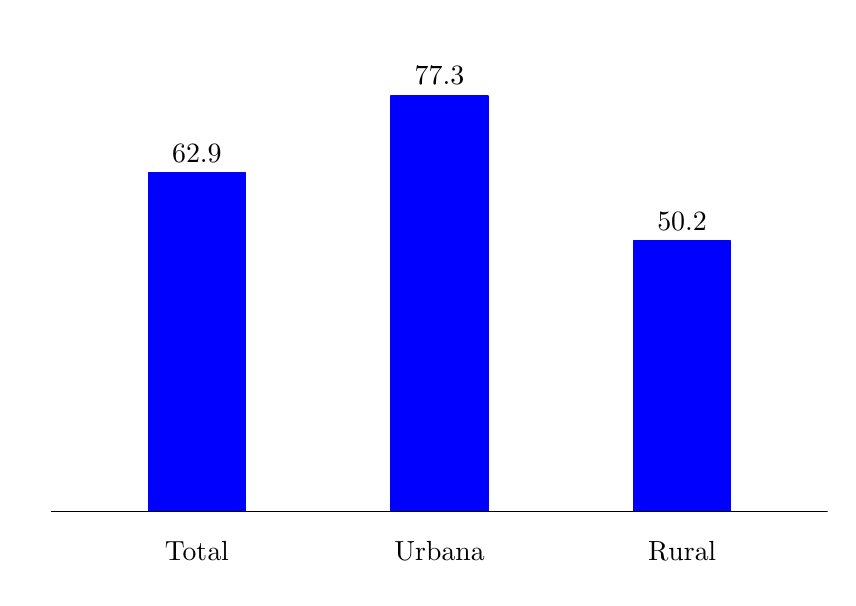
\begin{tikzpicture}[x=1pt,y=1pt]  % Created by tikzDevice version 0.7.0 on 2015-11-25 06:57:15
% !TEX encoding = UTF-8 Unicode
\definecolor[named]{fillColor}{rgb}{1.00,1.00,1.00}
\path[use as bounding box,fill=fillColor,fill opacity=0.00] (0,0) rectangle (289.08,198.74);
\begin{scope}
\path[clip] (  0.00,  0.00) rectangle (289.08,198.74);

\path[] (  0.00,  0.00) rectangle (289.08,198.74);
\end{scope}
\begin{scope}
\path[clip] (  0.00,  0.00) rectangle (289.08,198.74);

\path[] (  8.54, 16.35) rectangle (289.08,181.67);

\path[] ( 61.14, 16.35) --
	( 61.14,181.67);

\path[] (148.81, 16.35) --
	(148.81,181.67);

\path[] (236.48, 16.35) --
	(236.48,181.67);
\definecolor[named]{drawColor}{rgb}{0.00,0.00,1.00}
\definecolor[named]{fillColor}{rgb}{0.00,0.00,1.00}

\path[draw=drawColor,line width= 0.6pt,line join=round,fill=fillColor] ( 43.60, 23.87) rectangle ( 78.67,146.19);

\path[draw=drawColor,line width= 0.6pt,line join=round,fill=fillColor] (131.27, 23.87) rectangle (166.34,174.16);

\path[draw=drawColor,line width= 0.6pt,line join=round,fill=fillColor] (218.94, 23.87) rectangle (254.01,121.55);
\definecolor[named]{drawColor}{rgb}{0.00,0.00,0.00}
\definecolor[named]{fillColor}{rgb}{0.00,0.00,0.00}

\path[draw=drawColor,line width= 0.1pt,line join=round,fill=fillColor] (  8.54, 23.87) -- (289.08, 23.87);

\node[text=drawColor,anchor=base,inner sep=0pt, outer sep=0pt, scale=  1.01] at ( 61.14,150.15) {62.9};

\node[text=drawColor,anchor=base,inner sep=0pt, outer sep=0pt, scale=  1.01] at (148.81,178.11) {77.3};

\node[text=drawColor,anchor=base,inner sep=0pt, outer sep=0pt, scale=  1.01] at (236.48,125.51) {50.2};

\path[] (  8.54, 16.35) rectangle (289.08,181.67);
\end{scope}
\begin{scope}
\path[clip] (  0.00,  0.00) rectangle (289.08,198.74);

\path[] (  8.54, 16.35) --
	(  8.54,181.67);
\end{scope}
\begin{scope}
\path[clip] (  0.00,  0.00) rectangle (289.08,198.74);

\path[] (  8.54, 16.35) --
	(289.08, 16.35);
\end{scope}
\begin{scope}
\path[clip] (  0.00,  0.00) rectangle (289.08,198.74);

\path[] ( 61.14, 12.08) --
	( 61.14, 16.35);

\path[] (148.81, 12.08) --
	(148.81, 16.35);

\path[] (236.48, 12.08) --
	(236.48, 16.35);
\end{scope}
\begin{scope}
\path[clip] (  0.00,  0.00) rectangle (289.08,198.74);
\definecolor[named]{drawColor}{rgb}{0.00,0.00,0.00}

\node[text=drawColor,anchor=base,inner sep=0pt, outer sep=0pt, scale=  1.00] at ( 61.14,  6.04) {Total};

\node[text=drawColor,anchor=base,inner sep=0pt, outer sep=0pt, scale=  1.00] at (148.81,  6.04) {Urbana};

\node[text=drawColor,anchor=base,inner sep=0pt, outer sep=0pt, scale=  1.00] at (236.48,  6.04) {Rural};
\end{scope}
  \end{tikzpicture}}%
{%
 Instituto Nacional de Estadística} %
 
 \cajota{%
Partos con asistencia de personal de salud en los departamentos}%
{%
 El departamento de Guatemala  es donde se observa la mayor atención de partos\footnote{El indicador se calcula con los nacimientos de los cinco años anteriores a la encuesta.} por médico o ginecólogo (94.2\%), mientras que  el de Totonicapán, tiene el menor porcentaje (32.8\%).\\\\ 
Para el departamento de Quiché, uno de cada tres partos son atendidos por médico, mientras que en Huehuetenango y Alta Verapaz, poco más del 38\%.}%
{%
 Proporción de partos con asistencia de médico o ginecólogo} %
{%
 Républica de Guatemala, Encovi 2000, 2006 y 2014, en quetzales de cada año} %
{%
 \includegraphics[width=52\cuadri]{graficas/3_21.pdf}}%
{%
 Instituto Nacional de Estadística} %
 
 \cajita{%
Atención del parto en centros públicos}%
{%
 Nota: para los nacimientos de los cinco años anteriores a cada encuesta.}%
{%
 Proporción de partos con asistencia de médico o ginecólogo} %
{%
 Républica de Guatemala, Encovi 2000, 2006 y 2014, en quetzales de cada año} %
{%
 \begin{tikzpicture}[x=1pt,y=1pt]  % Created by tikzDevice version 0.7.0 on 2015-11-27 14:18:01
% !TEX encoding = UTF-8 Unicode
\definecolor[named]{fillColor}{rgb}{1.00,1.00,1.00}
\path[use as bounding box,fill=fillColor,fill opacity=0.00] (0,0) rectangle (289.08,198.74);
\begin{scope}
\path[clip] (  0.00,  0.00) rectangle (289.08,198.74);

\path[] (  0.00,  0.00) rectangle (289.08,198.74);
\end{scope}
\begin{scope}
\path[clip] (  0.00,  0.00) rectangle (289.08,198.74);

\path[] (  1.64, 17.78) rectangle (280.54,191.48);

\path[] (  1.64, 46.45) --
	(280.54, 46.45);

\path[] (  1.64, 88.01) --
	(280.54, 88.01);

\path[] (  1.64,129.56) --
	(280.54,129.56);

\path[] (  1.64,171.12) --
	(280.54,171.12);

\path[] (  1.64, 25.67) --
	(280.54, 25.67);

\path[] (  1.64, 67.23) --
	(280.54, 67.23);

\path[] (  1.64,108.78) --
	(280.54,108.78);

\path[] (  1.64,150.34) --
	(280.54,150.34);

\path[] ( 41.49, 17.78) --
	( 41.49,191.48);

\path[] (107.89, 17.78) --
	(107.89,191.48);

\path[] (174.30, 17.78) --
	(174.30,191.48);

\path[] (240.70, 17.78) --
	(240.70,191.48);
\definecolor[named]{drawColor}{rgb}{0.00,0.00,1.00}

\path[draw=drawColor,line width= 1.7pt,line join=round] ( 41.49, 62.94) --
	(107.89, 90.49) --
	(174.30,135.28) --
	(240.70,163.62);
\definecolor[named]{drawColor}{rgb}{0.00,0.00,0.00}

\node[text=drawColor,anchor=base,inner sep=0pt, outer sep=0pt, scale=  1.01] at ( 41.49, 51.07) {29.0};

\node[text=drawColor,anchor=base east,inner sep=0pt, outer sep=0pt, scale=  1.01] at (104.78, 90.49) {35.6};

\node[text=drawColor,anchor=base east,inner sep=0pt, outer sep=0pt, scale=  1.01] at (171.18,135.28) {46.4};

\node[text=drawColor,anchor=base,inner sep=0pt, outer sep=0pt, scale=  1.01] at (240.70,167.57) {53.2};
\definecolor[named]{fillColor}{rgb}{0.00,0.00,0.00}

\path[draw=drawColor,line width= 0.1pt,line join=round,fill=fillColor] (  1.64, 25.67) -- (280.54, 25.67);

\path[] (  1.64, 17.78) rectangle (280.54,191.48);
\end{scope}
\begin{scope}
\path[clip] (  0.00,  0.00) rectangle (289.08,198.74);

\path[] (  1.64, 17.78) --
	(  1.64,191.48);
\end{scope}
\begin{scope}
\path[clip] (  0.00,  0.00) rectangle (289.08,198.74);

\path[] (  0.00, 25.67) --
	(  1.64, 25.67);

\path[] (  0.00, 67.23) --
	(  1.64, 67.23);

\path[] (  0.00,108.78) --
	(  1.64,108.78);

\path[] (  0.00,150.34) --
	(  1.64,150.34);
\end{scope}
\begin{scope}
\path[clip] (  0.00,  0.00) rectangle (289.08,198.74);

\path[] (  1.64, 17.78) --
	(280.54, 17.78);
\end{scope}
\begin{scope}
\path[clip] (  0.00,  0.00) rectangle (289.08,198.74);

\path[] ( 41.49, 13.51) --
	( 41.49, 17.78);

\path[] (107.89, 13.51) --
	(107.89, 17.78);

\path[] (174.30, 13.51) --
	(174.30, 17.78);

\path[] (240.70, 13.51) --
	(240.70, 17.78);
\end{scope}
\begin{scope}
\path[clip] (  0.00,  0.00) rectangle (289.08,198.74);
\definecolor[named]{drawColor}{rgb}{0.00,0.00,0.00}

\node[text=drawColor,anchor=base,inner sep=0pt, outer sep=0pt, scale=  1.00] at ( 41.49,  2.85) {2000};

\node[text=drawColor,anchor=base,inner sep=0pt, outer sep=0pt, scale=  1.00] at (107.89,  2.85) {2006};

\node[text=drawColor,anchor=base,inner sep=0pt, outer sep=0pt, scale=  1.00] at (174.30,  2.85) {2011};

\node[text=drawColor,anchor=base,inner sep=0pt, outer sep=0pt, scale=  1.00] at (240.70,  2.85) {2014};
\end{scope}
  \end{tikzpicture}}%
{%
 Instituto Nacional de Estadística} %
 
 \cajita{%
Atención del parto en centros públicos por área de residencia}%
{%
 Para 2014, el 57.3\% de los partos atendidos en el área urbana fue en hospitales, centros y puestos de salud público, mientras que en el área rural, la relacion fue uno de cada dos partos fue atendido en hospitales, centros de salud y puestos de salud públicos. Tanto para el área urbana como para el área rural, la mayor proporción fue en hospitales públicos.}%
{%
 Proporción de partos atendidos en hospital, centro o puesto de salud público por área de residencia} %
{%
 Républica de Guatemala, Encovi 2000, 2006 y 2014, en quetzales de cada año} %
{%
 \begin{tikzpicture}[x=1pt,y=1pt]  \input{graficas/3_23.tex}  \end{tikzpicture}}%
{%
 Instituto Nacional de Estadística} %
 
 \cajota{%
Atención del parto en centros públicos en los departamentos}%
{%
 En los departamentos de Totonicapán y Quiché, menos de la tercera parte de los partos son atendidos en centros de salud público, que incluye puestos, centros y hospitales, y en Sololá y Huehuetenango, poco más del 35\%. Mientras que en los departamentos de Jutiapa, El Progreso y Sacatepéquez, más del 70\% de los partos son atendidos en centros públicos.  }%
{%
 Proporción de partos atendidos en hospital, centro o puesto de salud público por departamento} %
{%
 Républica de Guatemala, Encovi 2000, 2006 y 2014, en quetzales de cada año} %
{%
 \includegraphics[width=52\cuadri]{graficas/3_24.pdf}}%
{%
 Instituto Nacional de Estadística} %
 
 \cajita{%
Acceso a agua mejorada}%
{%
 Nota: incluye tubería dentro de la vivienda, tubería fuera de la vivienda pero en el terreno y chorro público. Para el año 2000, el 72.6\% de la población tenía acceso a mejores fuentes de abastecimiento de agua, que incluye acceso a agua por medio de tubería dentro y fuera de la vivienda y chorro público. De 2000 a 2006, el acceso a agua mejorada aumentó en más de seis puntos porcentuales, no obstante en 2011 se redujo a 75.3\%. Para 2014, se observó que el 77.8\% de los hogares tienen acceso a fuentes mejoradas de abastecimiento de agua.}%
{%
 Proporción de la población con acceso a fuentes mejoradas de abastecimiento de agua potable} %
{%
 Républica de Guatemala, Encovi 2000, 2006 y 2014, en quetzales de cada año} %
{%
 \begin{tikzpicture}[x=1pt,y=1pt]  % Created by tikzDevice version 0.7.0 on 2015-11-26 07:46:48
% !TEX encoding = UTF-8 Unicode
\definecolor[named]{fillColor}{rgb}{1.00,1.00,1.00}
\path[use as bounding box,fill=fillColor,fill opacity=0.00] (0,0) rectangle (289.08,198.74);
\begin{scope}
\path[clip] (  0.00,  0.00) rectangle (289.08,198.74);

\path[] (  0.00,  0.00) rectangle (289.08,198.74);
\end{scope}
\begin{scope}
\path[clip] (  0.00,  0.00) rectangle (289.08,198.74);

\path[] (  1.64, 17.78) rectangle (280.54,191.48);

\path[] (  1.64, 41.46) --
	(280.54, 41.46);

\path[] (  1.64, 73.05) --
	(280.54, 73.05);

\path[] (  1.64,104.63) --
	(280.54,104.63);

\path[] (  1.64,136.21) --
	(280.54,136.21);

\path[] (  1.64,167.80) --
	(280.54,167.80);

\path[] (  1.64, 25.67) --
	(280.54, 25.67);

\path[] (  1.64, 57.25) --
	(280.54, 57.25);

\path[] (  1.64, 88.84) --
	(280.54, 88.84);

\path[] (  1.64,120.42) --
	(280.54,120.42);

\path[] (  1.64,152.00) --
	(280.54,152.00);

\path[] (  1.64,183.59) --
	(280.54,183.59);

\path[] ( 41.49, 17.78) --
	( 41.49,191.48);

\path[] (107.89, 17.78) --
	(107.89,191.48);

\path[] (174.30, 17.78) --
	(174.30,191.48);

\path[] (240.70, 17.78) --
	(240.70,191.48);
\definecolor[named]{drawColor}{rgb}{0.00,0.00,1.00}

\path[draw=drawColor,line width= 1.7pt,line join=round] ( 41.49,128.63) --
	(107.89,147.90) --
	(174.30,137.16) --
	(240.70,145.00);
\definecolor[named]{drawColor}{rgb}{0.00,0.00,0.00}

\node[text=drawColor,anchor=base,inner sep=0pt, outer sep=0pt, scale=  1.01] at ( 41.49,116.76) {72.6};

\node[text=drawColor,anchor=base,inner sep=0pt, outer sep=0pt, scale=  1.01] at (107.89,151.85) {78.7};

\node[text=drawColor,anchor=base,inner sep=0pt, outer sep=0pt, scale=  1.01] at (174.30,125.29) {75.3};

\node[text=drawColor,anchor=base,inner sep=0pt, outer sep=0pt, scale=  1.01] at (240.70,148.96) {77.8};
\definecolor[named]{fillColor}{rgb}{0.00,0.00,0.00}

\path[draw=drawColor,line width= 0.1pt,line join=round,fill=fillColor] (  1.64, 25.67) -- (280.54, 25.67);

\path[] (  1.64, 17.78) rectangle (280.54,191.48);
\end{scope}
\begin{scope}
\path[clip] (  0.00,  0.00) rectangle (289.08,198.74);

\path[] (  1.64, 17.78) --
	(  1.64,191.48);
\end{scope}
\begin{scope}
\path[clip] (  0.00,  0.00) rectangle (289.08,198.74);

\path[] (  0.00, 25.67) --
	(  1.64, 25.67);

\path[] (  0.00, 57.25) --
	(  1.64, 57.25);

\path[] (  0.00, 88.84) --
	(  1.64, 88.84);

\path[] (  0.00,120.42) --
	(  1.64,120.42);

\path[] (  0.00,152.00) --
	(  1.64,152.00);

\path[] (  0.00,183.59) --
	(  1.64,183.59);
\end{scope}
\begin{scope}
\path[clip] (  0.00,  0.00) rectangle (289.08,198.74);

\path[] (  1.64, 17.78) --
	(280.54, 17.78);
\end{scope}
\begin{scope}
\path[clip] (  0.00,  0.00) rectangle (289.08,198.74);

\path[] ( 41.49, 13.51) --
	( 41.49, 17.78);

\path[] (107.89, 13.51) --
	(107.89, 17.78);

\path[] (174.30, 13.51) --
	(174.30, 17.78);

\path[] (240.70, 13.51) --
	(240.70, 17.78);
\end{scope}
\begin{scope}
\path[clip] (  0.00,  0.00) rectangle (289.08,198.74);
\definecolor[named]{drawColor}{rgb}{0.00,0.00,0.00}

\node[text=drawColor,anchor=base,inner sep=0pt, outer sep=0pt, scale=  1.00] at ( 41.49,  2.85) {2000};

\node[text=drawColor,anchor=base,inner sep=0pt, outer sep=0pt, scale=  1.00] at (107.89,  2.85) {2006};

\node[text=drawColor,anchor=base,inner sep=0pt, outer sep=0pt, scale=  1.00] at (174.30,  2.85) {2011};

\node[text=drawColor,anchor=base,inner sep=0pt, outer sep=0pt, scale=  1.00] at (240.70,  2.85) {2014};
\end{scope}
  \end{tikzpicture}}%
{%
 Instituto Nacional de Estadística} %
 
 \cajita{%
Acceso a agua mejorada por área de residencia}%
{%
 Nota: incluye tubería dentro de la vivienda, tubería fuera de la vivienda pero en el terreno y chorro público. Al desagregar por área de residencia se observa que es mayor el acceso a agua mejorada en el área urbana, ya que el 89.1\% tiene acceso a mejores fuentes de abastecimiento de agua, en comparación con el 64.4\% de población que tiene acceso en el área rural.}%
{%
 Proporción de partos con asistencia de médico o ginecólogo} %
{%
 Républica de Guatemala, Encovi 2000, 2006 y 2014, en quetzales de cada año} %
{%
 \begin{tikzpicture}[x=1pt,y=1pt]  \input{graficas/3_26.tex}  \end{tikzpicture}}%
{%
 Instituto Nacional de Estadística} %
 
 \cajota{%
Acceso a agua mejorada en los departamentos}%
{%
  Los departamentos con mayor acceso a mejores fuentes de abastecimiento de agua\footnote{Fuentes mejoradas de abastecimiento de agua potable incluye tubería tanto  dentro de la vivienda como  fuera pero en el terreno, y chorro público.} , son Guatemala, Sacatepéquez y Sololá, con más del 90\% de acceso. 
 
  Por otro lado, en el departamento de Alta Verapaz, menos de la mitad de la población tiene acceso a tubería dentro y fuera de la vivienda o  chorro público.}%
{%
 Proporción de partos con asistencia de médico o ginecólogo} %
{%
 Républica de Guatemala, Encovi 2000, 2006 y 2014, en quetzales de cada año} %
{%
 \includegraphics[width=52\cuadri]{graficas/3_27.pdf}}%
{%
 Instituto Nacional de Estadística} %
 
 \cajita{%
Acceso a saneamiento mejorado}%
{%
 Nota: incluye inodoro conectado a red de drenaje, inodoro conectado a fosa séptica y excusado lavable.}%
{%
 Proporción de partos con asistencia de médico o ginecólogo} %
{%
 Républica de Guatemala, Encovi 2000, 2006 y 2014, en quetzales de cada año} %
{%
 \begin{tikzpicture}[x=1pt,y=1pt]  % Created by tikzDevice version 0.9 on 2015-11-30 18:02:28
% !TEX encoding = UTF-8 Unicode
\definecolor{fillColor}{RGB}{255,255,255}
\path[use as bounding box,fill=fillColor,fill opacity=0.00] (0,0) rectangle (289.08,198.74);
\begin{scope}
\path[clip] (  0.00,  0.00) rectangle (289.08,198.74);

\path[] (  0.00,  0.00) rectangle (289.08,198.74);
\end{scope}
\begin{scope}
\path[clip] (  0.00,  0.00) rectangle (289.08,198.74);

\path[] (  1.64, 17.78) rectangle (280.54,191.48);

\path[] (  1.64, 42.59) --
	(280.54, 42.59);

\path[] (  1.64, 98.99) --
	(280.54, 98.99);

\path[] (  1.64,155.39) --
	(280.54,155.39);

\path[] (  1.64, 70.79) --
	(280.54, 70.79);

\path[] (  1.64,127.19) --
	(280.54,127.19);

\path[] (  1.64,183.59) --
	(280.54,183.59);

\path[] ( 41.49, 17.78) --
	( 41.49,191.48);

\path[] (107.89, 17.78) --
	(107.89,191.48);

\path[] (174.30, 17.78) --
	(174.30,191.48);

\path[] (240.70, 17.78) --
	(240.70,191.48);
\definecolor{drawColor}{RGB}{0,0,255}

\path[draw=drawColor,line width= 1.7pt,line join=round] ( 41.49, 94.48) --
	(107.89,152.57) --
	(174.30,161.03) --
	(240.70,173.86);
\definecolor{drawColor}{RGB}{0,0,0}

\node[text=drawColor,anchor=base,inner sep=0pt, outer sep=0pt, scale=  1.01] at ( 41.49, 82.61) {44.2};

\node[text=drawColor,anchor=base east,inner sep=0pt, outer sep=0pt, scale=  1.01] at (104.78,152.57) {54.5};

\node[text=drawColor,anchor=base east,inner sep=0pt, outer sep=0pt, scale=  1.01] at (171.18,161.03) {56.0};

\node[text=drawColor,anchor=base,inner sep=0pt, outer sep=0pt, scale=  1.01] at (240.70,177.82) {58.3};

\path[draw=drawColor,line width= 0.1pt,line join=round] (  1.64, 25.67) -- (280.54, 25.67);

\path[] (  1.64, 17.78) rectangle (280.54,191.48);
\end{scope}
\begin{scope}
\path[clip] (  0.00,  0.00) rectangle (289.08,198.74);

\path[] (  1.64, 17.78) --
	(  1.64,191.48);
\end{scope}
\begin{scope}
\path[clip] (  0.00,  0.00) rectangle (289.08,198.74);

\path[] (  0.00, 70.79) --
	(  1.64, 70.79);

\path[] (  0.00,127.19) --
	(  1.64,127.19);

\path[] (  0.00,183.59) --
	(  1.64,183.59);
\end{scope}
\begin{scope}
\path[clip] (  0.00,  0.00) rectangle (289.08,198.74);

\path[] (  1.64, 17.78) --
	(280.54, 17.78);
\end{scope}
\begin{scope}
\path[clip] (  0.00,  0.00) rectangle (289.08,198.74);

\path[] ( 41.49, 13.51) --
	( 41.49, 17.78);

\path[] (107.89, 13.51) --
	(107.89, 17.78);

\path[] (174.30, 13.51) --
	(174.30, 17.78);

\path[] (240.70, 13.51) --
	(240.70, 17.78);
\end{scope}
\begin{scope}
\path[clip] (  0.00,  0.00) rectangle (289.08,198.74);
\definecolor{drawColor}{RGB}{0,0,0}

\node[text=drawColor,anchor=base,inner sep=0pt, outer sep=0pt, scale=  1.00] at ( 41.49,  2.85) {2000};

\node[text=drawColor,anchor=base,inner sep=0pt, outer sep=0pt, scale=  1.00] at (107.89,  2.85) {2006};

\node[text=drawColor,anchor=base,inner sep=0pt, outer sep=0pt, scale=  1.00] at (174.30,  2.85) {2011};

\node[text=drawColor,anchor=base,inner sep=0pt, outer sep=0pt, scale=  1.00] at (240.70,  2.85) {2014};
\end{scope}
  \end{tikzpicture}}%
{%
 Instituto Nacional de Estadística} %
 
 \cajita{%
Acceso a saneamiento mejorado por área de residencia}%
{%
 Aunque en promedio casi el 60\% de la población tiene acceso a saneamiento mejorado\footnote{Incluye inodoro conectado a red de drenaje, inodoro conectado a fosa séptica y excusado lavable}, al desagregar por área de residencia se observa que para el área rural, menos del 30\% de los hogares tienen acceso, en comparación con el 83.0\% del área urbana.}%
{%
 Proporción de la población con acceso a servicios de saneamiento mejorados por área de residencia} %
{%
 Républica de Guatemala, Encovi 2000, 2006 y 2014, en quetzales de cada año} %
{%
 \begin{tikzpicture}[x=1pt,y=1pt]  \input{graficas/3_29.tex}  \end{tikzpicture}}%
{%
 Instituto Nacional de Estadística} %
 
 \cajota{%
Acceso a saneamiento mejorado en los departamentos}%
{%
 El 21.4\% de los hogares en Alta Verapaz y el 30.1\% en Totonicapán tiene acceso a saneamiento mejorado, mientras que en los departamentos de Guatemala y Sacatepéquez, casi el 90\% de los hogares cuenta con servicios de saneamiento mejorados.}%
{%
 Proporción de la población con acceso a servicios de saneamiento mejorados } %
{%
 Républica de Guatemala, Encovi 2000, 2006 y 2014, en quetzales de cada año} %
{%
 \includegraphics[width=52\cuadri]{graficas/3_30.pdf}}%
{%
 Instituto Nacional de Estadística} %
 